\setcounter{chapter}{4}
\chapter{Kết quả}

\section{Về môi trường hiện thực và nền tảng Moodle}

Nhóm đã cài đặt thành công môi trường máy chủ web sử dụng LAMP Stack, cài đặt được Moodle và cơ sở dữ liệu để phục vụ cho việc xây dựng công cụ EHAT.

\section{Về công cụ EHAT}

\subsection{So sánh EHAT với hai công cụ Analytics graphs và Quiz Analytics}

\subsubsection{Giống nhau}

\begin{itemize}
	\item Đều phân tích số liệu từ cơ sở dữ liệu của Moodle.
	\item EHAT và Analytics graphs mô tả được điểm số của học viên.
	\item Đều đánh giá được sự tương tác của học viên với khóa học.
\end{itemize}

\subsubsection{Khác nhau}

\begin{itemize}
	\item EHAT có thêm chức năng đánh giá chi tiết năng lực của từng học viên.
	\item EHAT mô tả được số lần truy cập vào các tài nguyên của từng học viên.
	\item EHAT cho phép giáo viên thêm tài liệu tham khảo.
	\item EHAT có thêm chức năng xem lại khóa học cho học viên.
\end{itemize}

Các chức năng mà EHAT hiện thực được nhắm đến hai đối tượng là GV và HV, chúng ta sẽ cùng xem xét kết quả của từng đối tượng mà EHAT đã làm được.

\vskip 5cm
\subsection{Chức năng của EHAT đối với GV}

\begin{itemize}
	\item Thứ nhất, nhóm đã hiện thực được biểu đồ mạng nhện nhằm đánh giá được chi tiết năng lực của từng học viên đồng thời có thêm chức năng so sánh hai học viên với nhau.
	
	\begin{center}
		\begin{figure}[htp]
			\begin{center}
				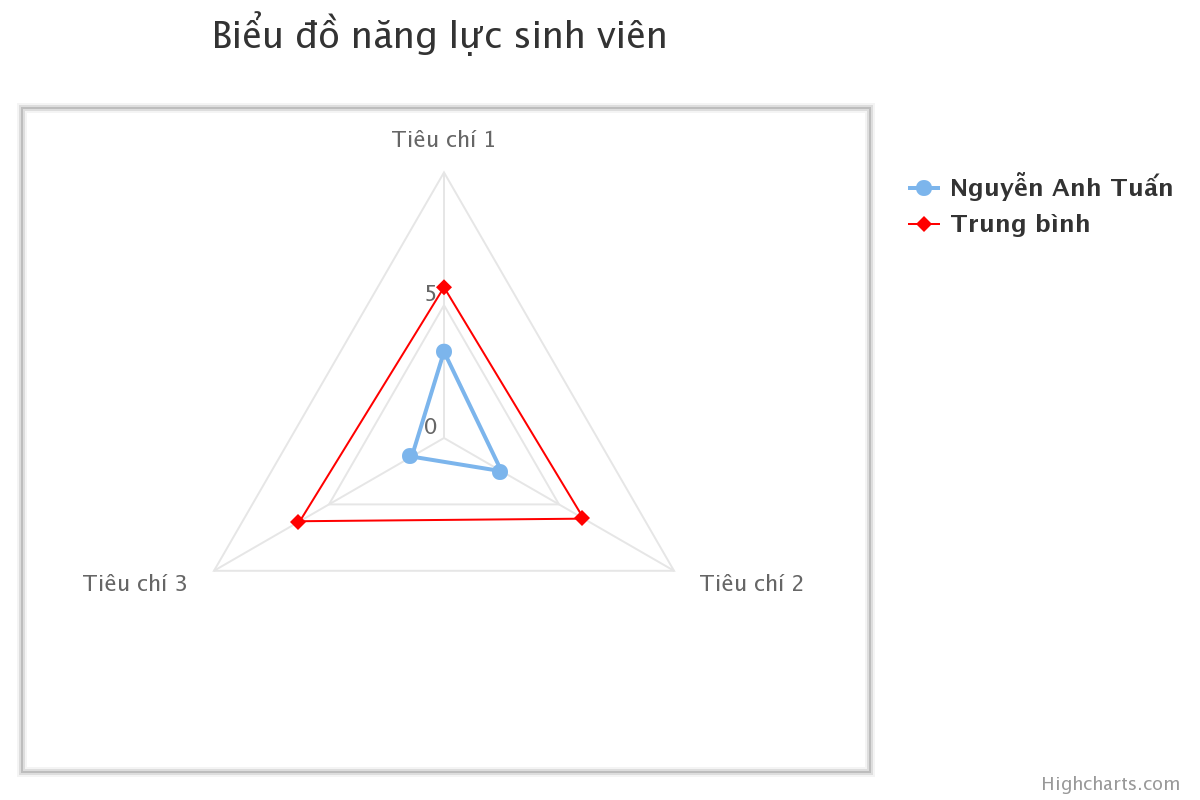
\includegraphics[width=0.8\linewidth]{img/22}
			\end{center}
			\caption{Giao diện biểu đồ mạng nhện}
			\label{refhinh70}
		\end{figure}
	\end{center}

	\begin{center}
		\begin{figure}[htp]
			\begin{center}
				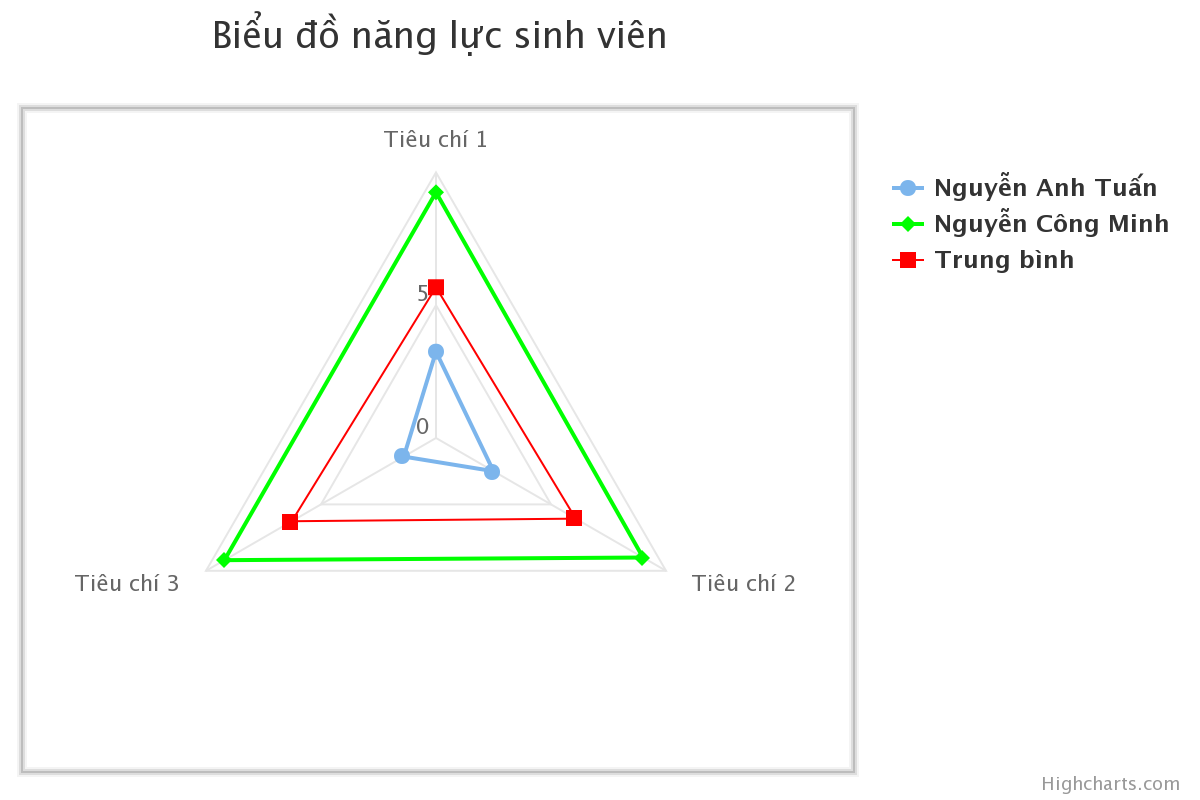
\includegraphics[width=0.8\linewidth]{img/25}
			\end{center}
			\caption{Biểu đồ so sánh 2 học viên}
			\label{refhinh71}
		\end{figure}
	\end{center}
	
	\vskip 5cm
	\item Thứ hai, chúng em đã thống kê được số lượt truy cập cũng như là không truy cập của học viên đối với một hạng mục cụ thể nào đó. Kết quả được hiển thị như hình sau
	
	\begin{center}
		\begin{figure}[htp]
			\begin{center}
				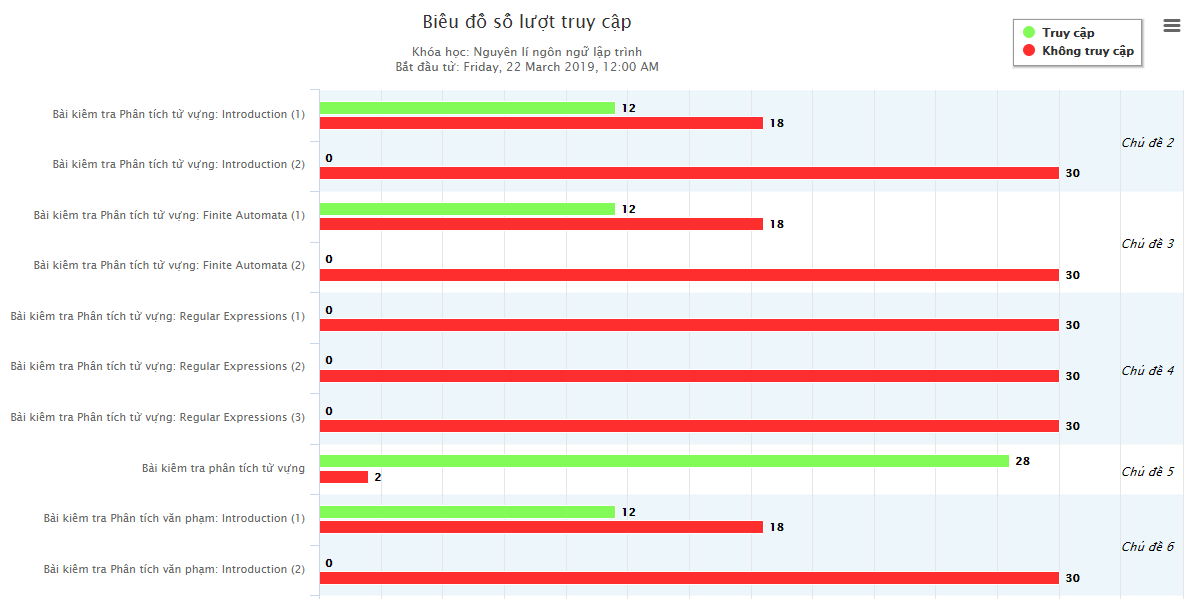
\includegraphics[width=1\linewidth]{img/27}
			\end{center}
			\caption{Biểu đồ cột ngang}
			\label{refhinh72}
		\end{figure}
	\end{center}

	\item Thứ ba, xây dựng thành công được chức năng nhằm đánh giá thái độ học tập của học viên dựa vào biểu đồ phân phối lượt truy cập của từng học viên.
	
	\begin{center}
		\begin{figure}[htp]
			\begin{center}
				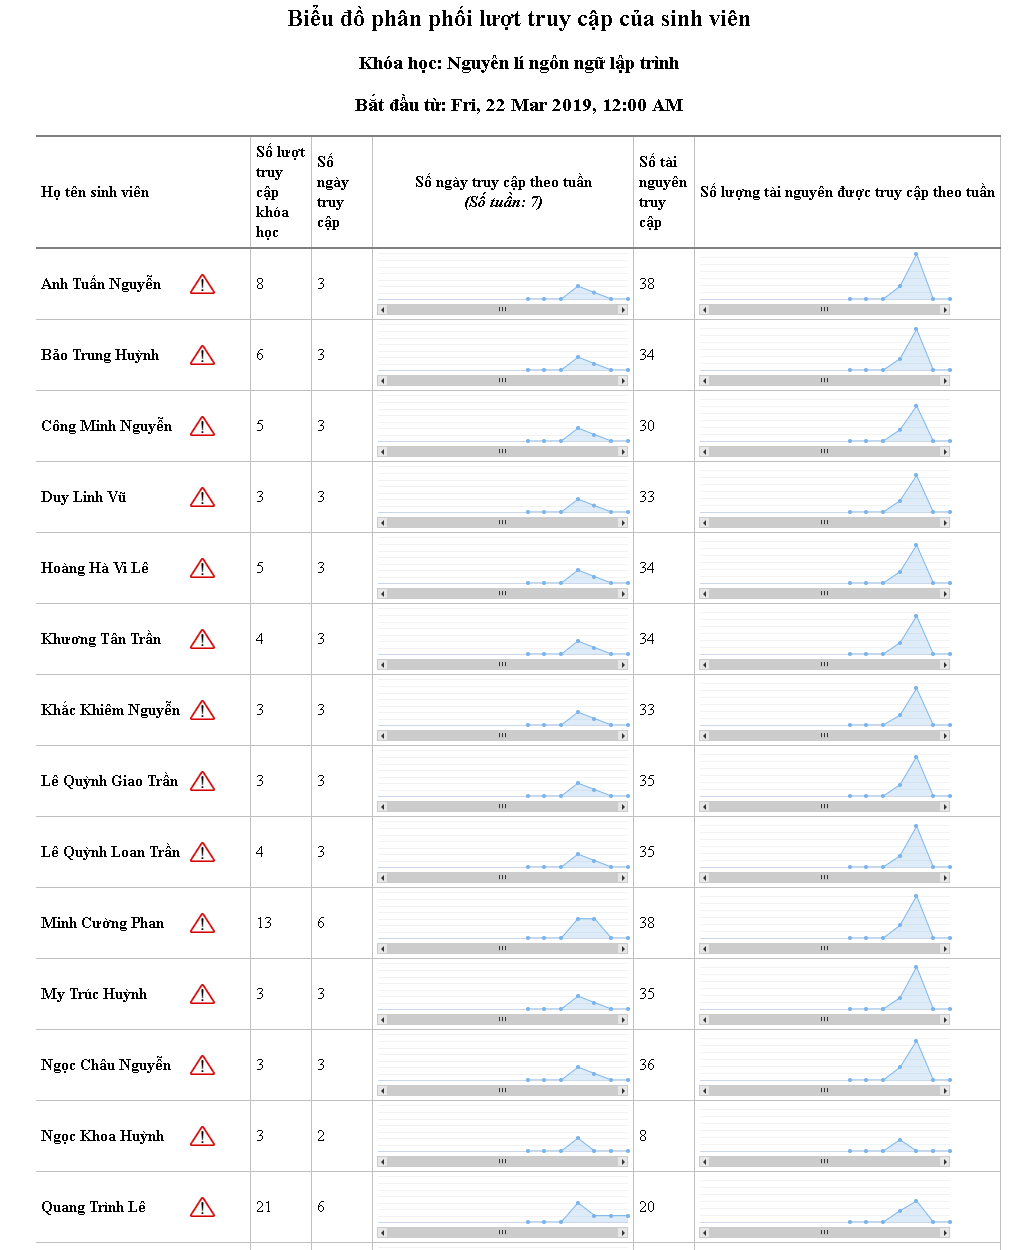
\includegraphics[width=0.6\linewidth]{img/29}
			\end{center}
			\caption{Biểu đồ phân phối lượt truy cập của HV}
			\label{refhinh73}
		\end{figure}
	\end{center}

	\begin{center}
		\begin{figure}[htp]
			\begin{center}
				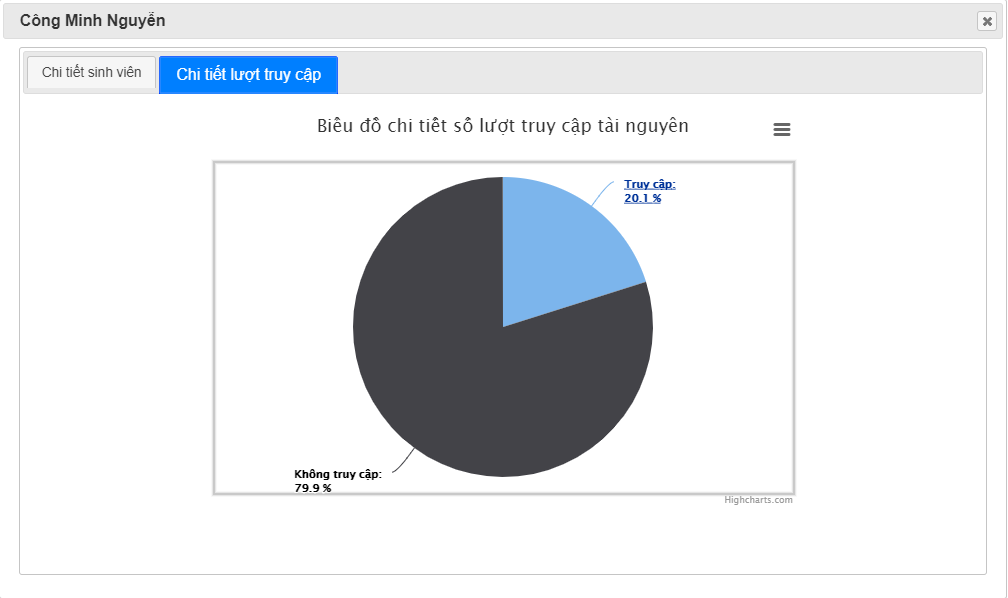
\includegraphics[width=0.8\linewidth]{img/41}
			\end{center}
			\caption{Biểu đồ thể hiện phần trăm truy cập}
			\label{refhinh74}
		\end{figure}
	\end{center}

	\begin{center}
		\begin{figure}[htp]
			\begin{center}
				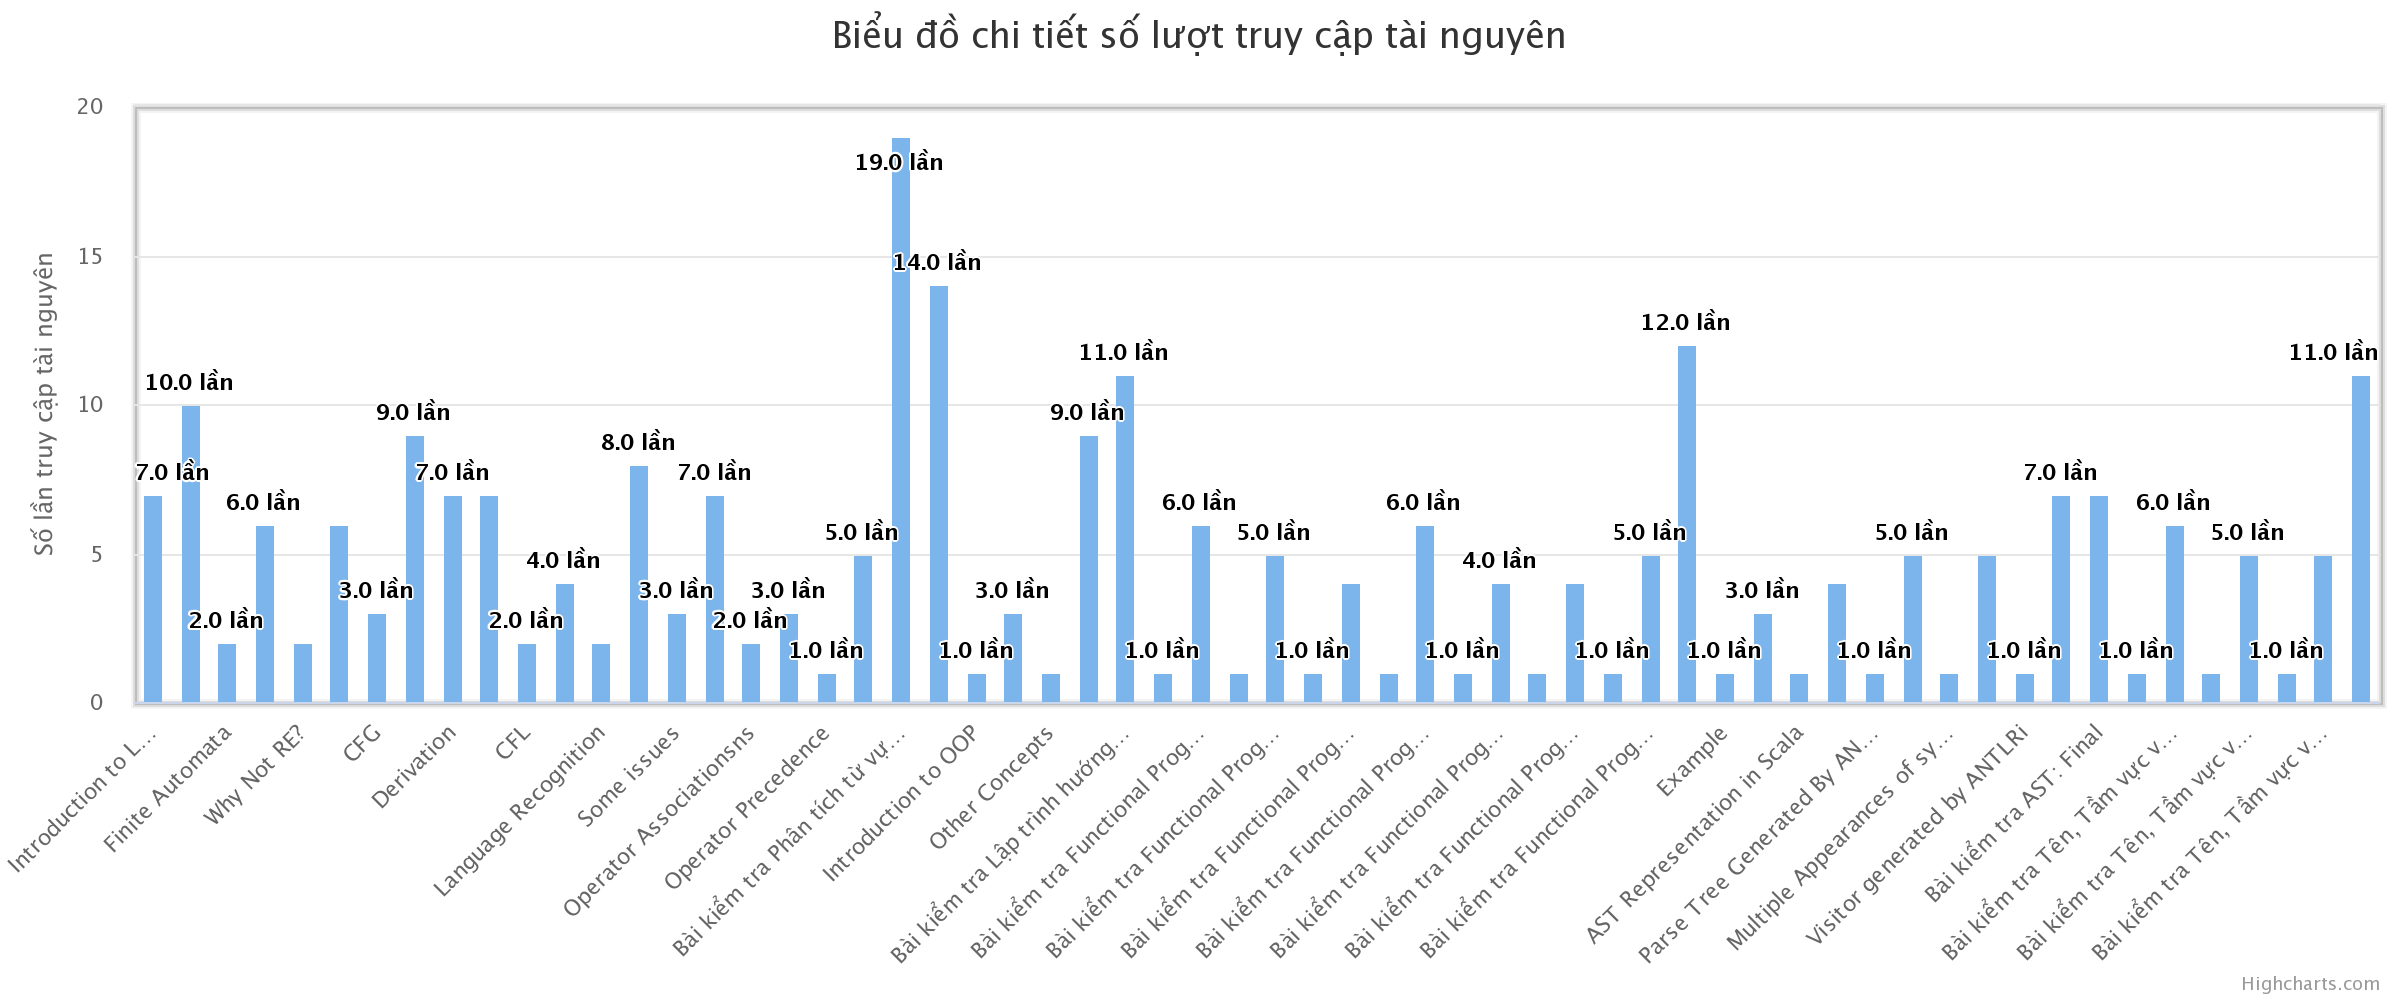
\includegraphics[width=1\linewidth]{img/50}
			\end{center}
			\caption{Biểu đồ thể hiện chi tiết số lần truy cập của học viên}
			\label{refhinh88}
		\end{figure}
	\end{center}

	\vskip 5cm
	\item Chức năng thứ tư mà nhóm hiện thực thành công đó là mô tả được hoạt động của học viên theo từng khung giờ trong ngày
	\begin{center}
		\begin{figure}[htp]
			\begin{center}
				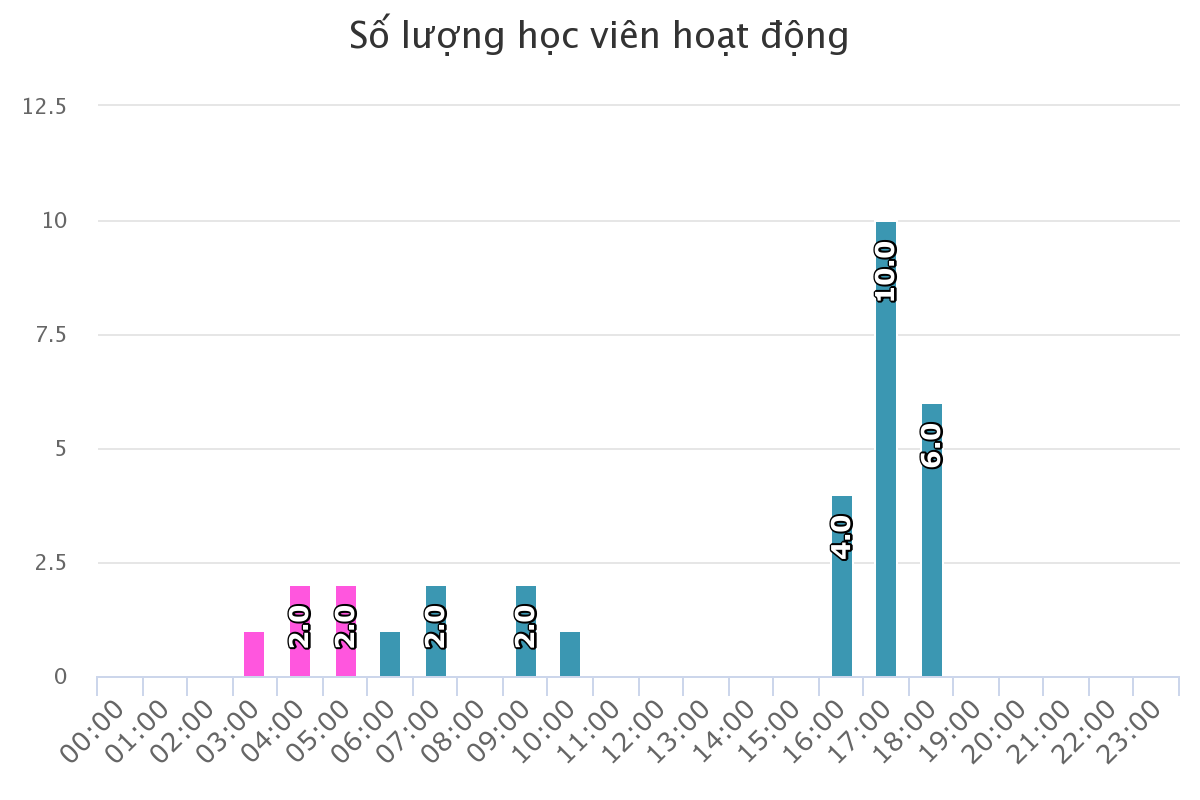
\includegraphics[width=0.8\linewidth]{img/51}
			\end{center}
			\caption{Biểu đồ số lượng học viên hoạt động theo khung giờ}
			\label{refhinh89}
		\end{figure}
	\end{center}

	\begin{center}
		\begin{figure}[htp]
			\begin{center}
				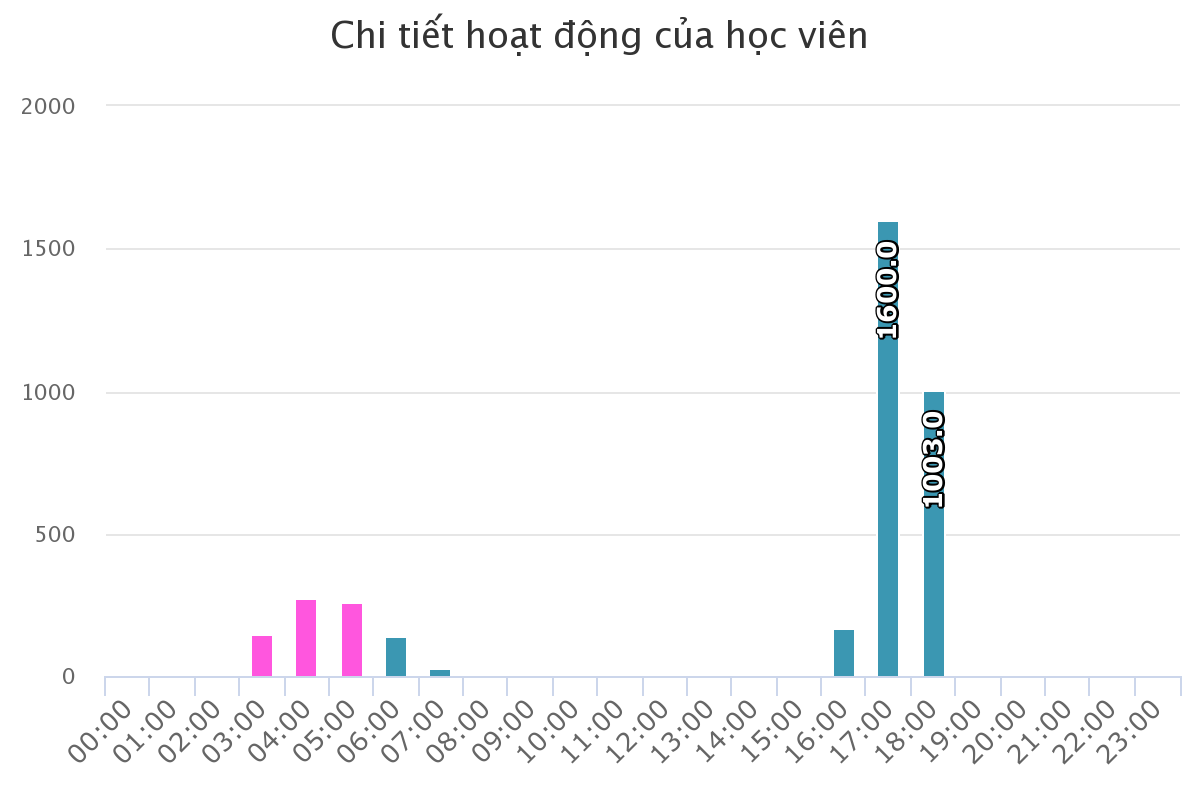
\includegraphics[width=0.8\linewidth]{img/52}
			\end{center}
			\caption{Biểu đồ số lượng học viên hoạt động theo khung giờ}
			\label{refhinh90}
		\end{figure}
	\end{center}
	
	\vskip 5cm
	\item Chức năng cuối cùng mà nhóm xây dựng được cho giảng viên đó là bảng hỗ trợ cho giảng viên thêm tài liệu tham khảo.
	
	\begin{center}
		\begin{figure}[htp]
			\begin{center}
				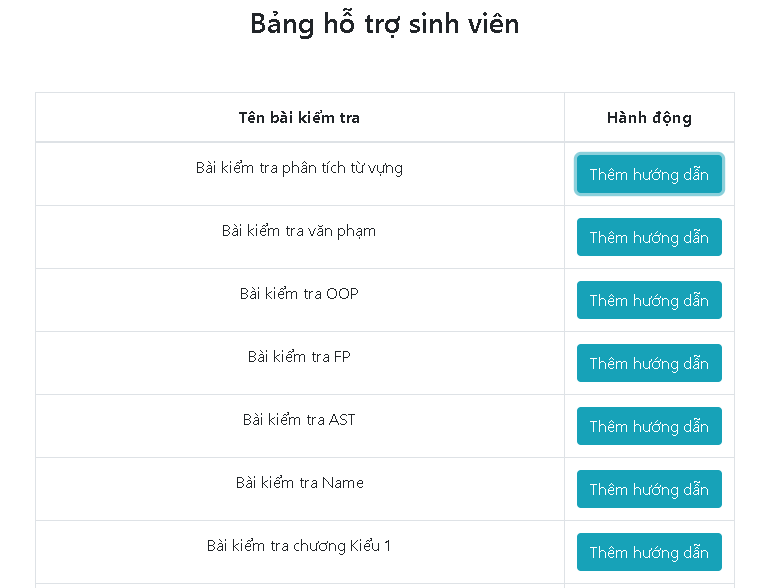
\includegraphics[width=0.6\linewidth]{img/30}
			\end{center}
			\caption{Chức năng cuối cùng dành cho GV}
			\label{refhinh75}
		\end{figure}
	\end{center}

	\begin{center}
		\begin{figure}[htp]
			\begin{center}
				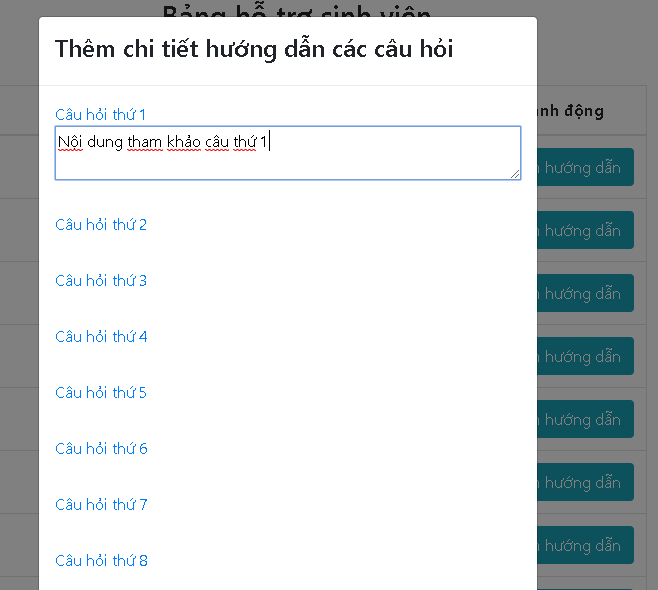
\includegraphics[width=0.6\linewidth]{img/31}
			\end{center}
			\caption{Chức năng cuối cùng dành cho GV}
			\label{refhinh76}
		\end{figure}
	\end{center}

\end{itemize}

\vskip 6cm
\subsection{Chức năng của EHAT đối với HV}

Đối với HV nhóm đã xây dựng được một chức năng nhằm giúp cho HV có thể tham khảo lại chi tiết bài kiểm tra mà mình đã làm ở lần cuối cùng.

\begin{center}
	\begin{figure}[htp]
		\begin{center}
			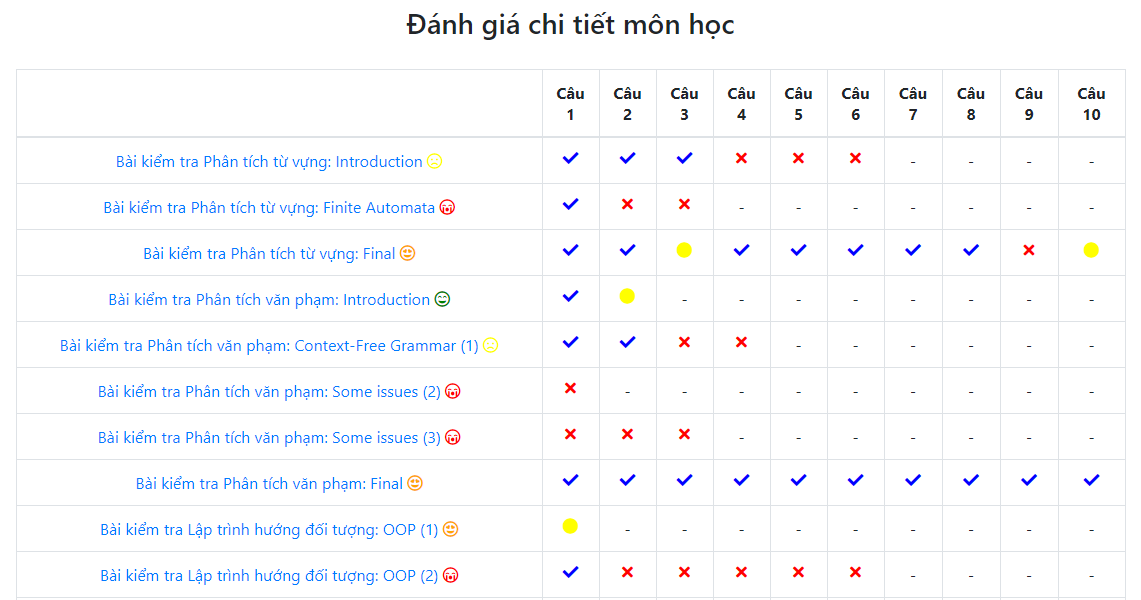
\includegraphics[width=0.8\linewidth]{img/33}
		\end{center}
		\caption{Bảng xem lại khóa học của học viên}
		\label{refhinh77}
	\end{figure}
\end{center}

Nội dung chi tiết của từng câu hỏi.

\begin{center}
	\begin{figure}[htp]
		\begin{center}
			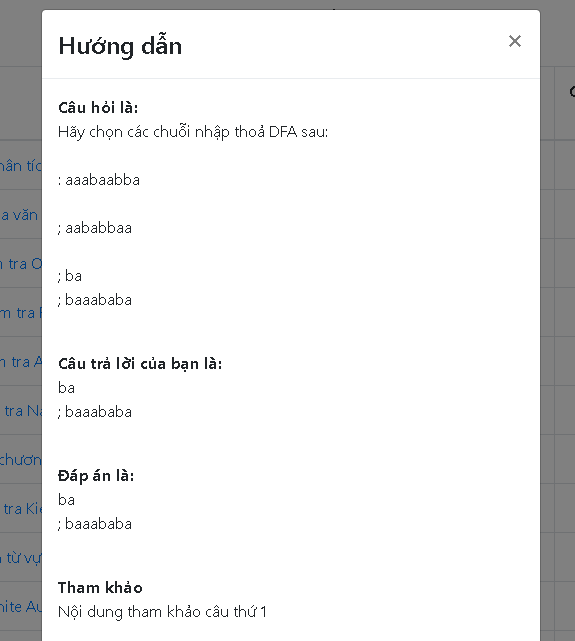
\includegraphics[width=0.5\linewidth]{img/34}
		\end{center}
		\caption{Nội dung chi tiết của từng câu hỏi}
		\label{refhinh78}
	\end{figure}
\end{center}
